\documentclass[border=10pt]{standalone}
\usepackage[svgnames]{xcolor}
\usepackage{amsmath}
\usepackage{pgfplots}
\pgfplotsset{compat=newest}
\usepackage[sfdefault]{FiraSans}
\usepackage{FiraMono}
\renewcommand*\familydefault{\sfdefault}
\begin{document}
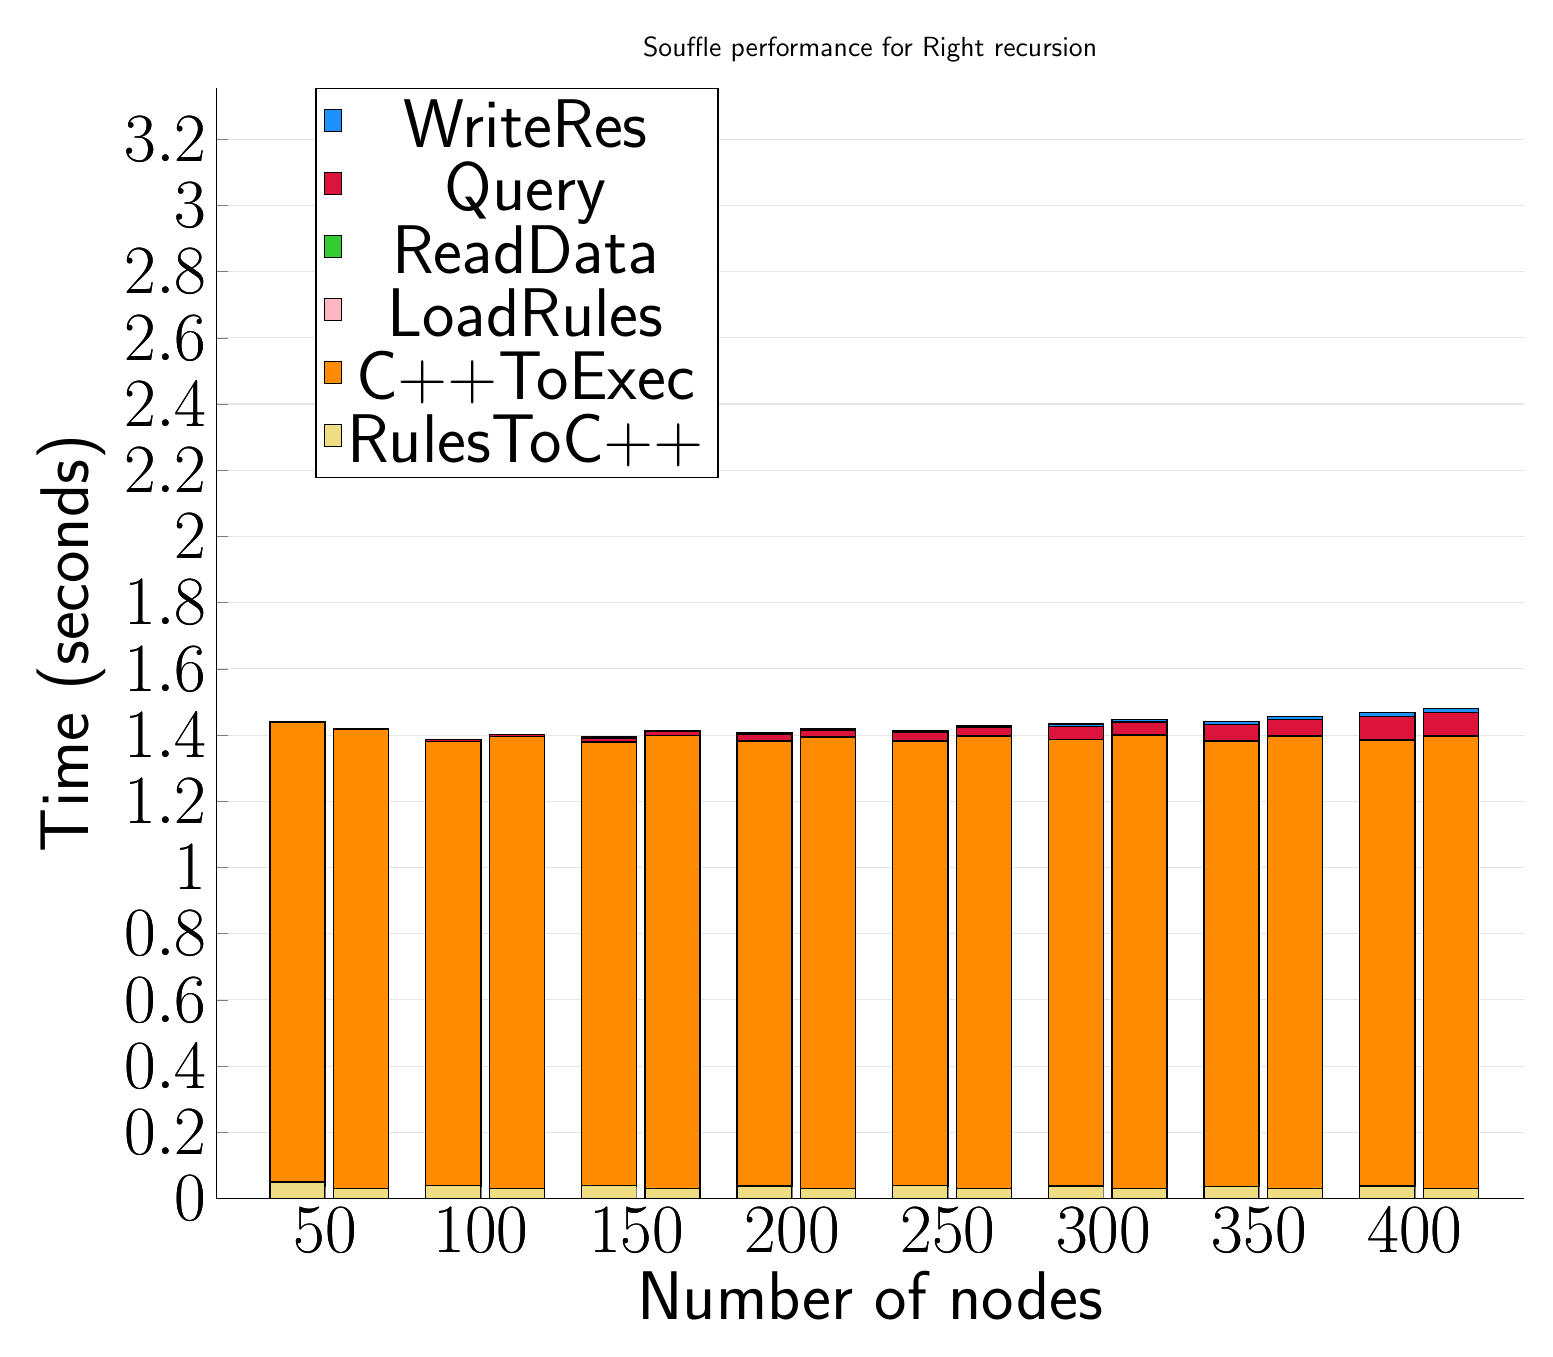
\begin{tikzpicture}
\begin{axis}[
   ybar stacked,
   title={Souffle performance for Right recursion},
   bar shift=-10pt,
   width=1.5\textwidth,
   bar width=0.7cm,
   ymajorgrids, tick align=inside,
   major grid style={draw=gray!20},
   xtick=data,
   ymin=0, ymax=3.3549999952316285,
   axis x line*=bottom,
   axis y line*=left,
   enlarge x limits=0.1,
   legend style={
       at={(0.23, 1)},
       anchor=north,
       legend columns=1,
       font=\Huge,
   },
   ylabel={Time (seconds)},
   xlabel={Number of nodes},
   label style={font=\Huge},
   tick label style={font=\Huge},
]
\addlegendimage{fill=DodgerBlue, draw=black, line width=0.2pt}
\addlegendentry{WriteRes}
\addlegendimage{fill=Crimson, draw=black, line width=0.2pt}
\addlegendentry{Query}
\addlegendimage{fill=LimeGreen, draw=black, line width=0.2pt}
\addlegendentry{ReadData}
\addlegendimage{fill=LightPink, draw=black, line width=0.2pt}
\addlegendentry{LoadRules}
\addlegendimage{fill=DarkOrange, draw=black, line width=0.2pt}
\addlegendentry{C++ToExec}
\addlegendimage{fill=LightGoldenrod, draw=black, line width=0.2pt}
\addlegendentry{RulesToC++}
\addplot +[fill=LightGoldenrod, draw=black, line width=0.5pt] coordinates {
    (50, 0.04999997615814209)
    (100, 0.04000000953674317)
    (150, 0.04000000953674317)
    (200, 0.0380000114440918)
    (250, 0.04000000953674317)
    (300, 0.03799998760223389)
    (350, 0.03700001239776611)
    (400, 0.037999963760375975)
};
\addplot +[fill=DarkOrange, draw=black, line width=0.5pt] coordinates {
    (50, 1.3880000352859496)
    (100, 1.3399999856948852)
    (150, 1.3390000104904174)
    (200, 1.3429999828338623)
    (250, 1.3419999599456787)
    (300, 1.3480000019073486)
    (350, 1.3440000057220458)
    (400, 1.3460000276565551)
};
\addplot +[fill=LightPink, draw=black, line width=0.5pt] coordinates {
    (50, 1.12167e-05)
    (100, 0.0)
    (150, 0.0)
    (200, 0.0)
    (250, 0.0)
    (300, 0.0)
    (350, 0.0)
    (400, 0.0)
};
\addplot +[fill=LimeGreen, draw=black, line width=0.5pt] coordinates {
    (50, 0.00042980400000000005)
    (100, 0.0006039417999999999)
    (150, 0.0007992750000000001)
    (200, 0.0009659717)
    (250, 0.001142891)
    (300, 0.0013229788)
    (350, 0.001465708)
    (400, 0.0018611639999999998)
};
\addplot +[fill=Crimson, draw=black, line width=0.5pt] coordinates {
    (50, 0.0012754349999999997)
    (100, 0.005270263)
    (150, 0.011474809999999998)
    (200, 0.02006107)
    (250, 0.026215)
    (300, 0.03936167)
    (350, 0.04887271)
    (400, 0.07001754)
};
\addplot +[fill=DodgerBlue, draw=black, line width=0.5pt] coordinates {
    (50, 0.0004822750999999999)
    (100, 0.0014212629999999996)
    (150, 0.0027339169999999998)
    (200, 0.004260504)
    (250, 0.005205682)
    (300, 0.007322184999999999)
    (350, 0.008872413000000001)
    (400, 0.012396160000000002)
};
\end{axis}
\begin{axis}[
   ybar stacked,
   bar shift=13pt,
   width=1.5\textwidth,
   bar width=0.7cm,
   ymajorgrids, tick align=inside,
   major grid style={draw=none},
   xtick=data,
   ymin=0, ymax=3.3549999952316285,
   axis x line*=none,
   axis y line*=none,
   enlarge x limits=0.1,
   label style={font=\Huge},
   tick label style={font=\Huge},
]
\addplot +[fill=LightGoldenrod, draw=black, line width=0.5pt] coordinates {
    (50, 0.031000000000000007)
    (100, 0.030000000000000006)
    (150, 0.030000000000000006)
    (200, 0.030000000000000006)
    (250, 0.030000000000000006)
    (300, 0.030000000000000006)
    (350, 0.030000000000000006)
    (400, 0.030000000000000006)
};
\addplot +[fill=DarkOrange, draw=black, line width=0.5pt] coordinates {
    (50, 1.3870000000000005)
    (100, 1.3649999999999998)
    (150, 1.3680000000000003)
    (200, 1.364)
    (250, 1.367)
    (300, 1.3690000000000002)
    (350, 1.3670000000000002)
    (400, 1.3670000000000004)
};
\addplot +[fill=LightPink, draw=black, line width=0.5pt] coordinates {
    (50, 1.11e-05)
    (100, 0.0)
    (150, 0.0)
    (200, 0.0)
    (250, 0.0)
    (300, 0.0)
    (350, 0.0)
    (400, 0.0)
};
\addplot +[fill=LimeGreen, draw=black, line width=0.5pt] coordinates {
    (50, 0.00042899999999999997)
    (100, 0.000603)
    (150, 0.0007983)
    (200, 0.0009653999999999999)
    (250, 0.0011419)
    (300, 0.0013221)
    (350, 0.0014648)
    (400, 0.0017973)
};
\addplot +[fill=Crimson, draw=black, line width=0.5pt] coordinates {
    (50, 0.0012752)
    (100, 0.005269500000000001)
    (150, 0.0114678)
    (200, 0.0200389)
    (250, 0.026190700000000004)
    (300, 0.039286600000000005)
    (350, 0.04879399999999999)
    (400, 0.06986789999999998)
};
\addplot +[fill=DodgerBlue, draw=black, line width=0.5pt] coordinates {
    (50, 0.00048130000000000004)
    (100, 0.0014197999999999997)
    (150, 0.0027275)
    (200, 0.0042571)
    (250, 0.0051936000000000005)
    (300, 0.007281900000000001)
    (350, 0.008761)
    (400, 0.012331400000000001)
};
\end{axis}
\end{tikzpicture}

\end{document}
